Redes Adhoc Móveis (\textit{MANETs}) são especialmente notáveis pela sua capacidade
de auto-organização e auto-configuração. Por definição, MANETs não contam com
estruturas fixas, sendo compostas por nós móveis tais como celulares, PDAs,
tablets e laptops, que se comunicam exclusivamente com tecnologia sem fio. Serviços
como roteamento e comunicação multi-salto são feitos contando com a cooperação
dos nós pertencentes à rede, mas nem todos podem ou precisam colaborar para todos
os serviços. A utilidade desse tipo de rede vai desde serviços militares até aplicações
de emergência e resgate \cite{manet-def}.

O avanço nas pesquisas de protocolos tem conferido mais confiabilidade e segurança
para redes MANET, permitindo a expansão de seu uso em vários níveis. Muitas das
barreiras e desafios identificados na última década já foram superadas ou apresentaram
uma melhora expressiva \cite{manet-state}.

Os problemas de roteamento foram resolvidos por protocolos relativamente recentes
como \textit{AdHoc On-Demand Distance Vector} (AODV) \cite{aodv} e
\textit{Dynamic Source Routing} (DSR) \cite{dsr}, permitindo que a transmissão de
mensagens ocorra em redes que exigem multi-salto. A Qualidade de Serviço é
frequentemente abordada em vários novos protocolos, \cite{qos1} e \cite{qos2}
demonstram algumas pesquisas nessa área. Segurança e consumo de energia são
preocupações constantes na nova geração de protocolos, fazendo com que a rede
evolua nesses aspectos a cada ano. No quesito controle de acesso ao meio, os
padrões de comunicação sem fio presentes na camada de enlace são utilizados,
como o IEEE 802.11 \cite{802-11}, o IEEE 802.15.4 \cite{802-15}, o IEEE 802.16
\cite{802-16} e o IEEE 802.22 \cite{802-22}.

A evolução dos protocolos de tradução de nomes tem sido tímida em MANETs. Do
modo como foi projetado em 1987 \cite{rfc1035}, o protocolo original do DNS é
altamente dependente de infraestrutura. Sua especificação prevê uma hierarquia rígida,
sua segurança e confiabilidade parte do pressuposto de servidores estáveis e de
uma rede com pouca volatilidade.

\begin{figure}[h!]
    \centering
    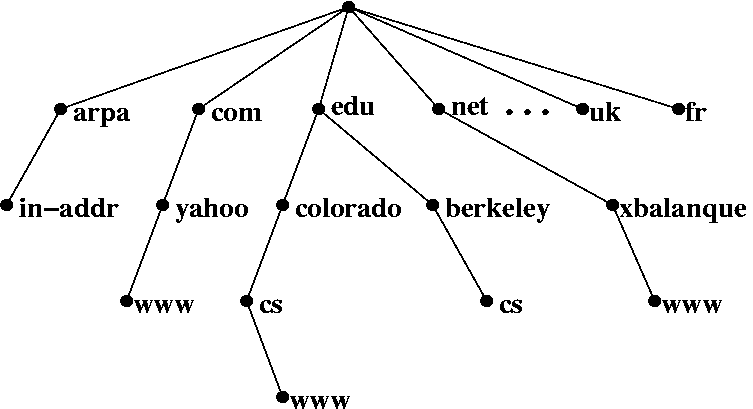
\includegraphics[width=0.7\textwidth]{figures/dns-1}
    \caption{Estrutura original do DNS}
    \label{dns}
\end{figure}

Como mostrado na figura \ref{dns}, o DNS foi especificado para usar servidores
estáticos e confiáveis. A raiz dessa árvore é chamado de Servidor Raiz
\cite{rfc1035}, e atualmente existem 13 cópias oficiais desse servidor espalhados
pelo mundo para garantir redundância \cite{iana}. Abaixo da raiz estão os
\textit{Top Level Domains} (TLDs); por motivos de segurança são exigidos pelo
menos dois servidores redundantes por TLD, mas na prática um servidor principal
conta com pelo menos outros dois servidores secundários. Abaixo dos TLDs estão
os \textit{Second Level Domains} (SLDs), que são subordinados aos TLDs e também
precisam ter pelo menos um servidor de redundância. Abaixo deles estão os subdomínios,
que, apesar de serem servidores, não necessariamente traduzem nomes, e a IANA não
regulamenta um número mínimo de redundância sobre eles. Um domínio qualificado é
um caminho reverso dos rótulos de um subdomínio até a raiz.

A configuração de cada um desses servidores (tanto TLDs quanto SLDs) é feita por
um arquivo que contém todos os nomes, traduções e configurações daquela zona -- 
isto é, o nó raiz precisa saber as traduções para todos os nós nos TLDs, cada nó
TLD é responsável pelos SLDs abaixo dele, e cada SLD é responsável pelos próprios
subdomínios. O arquivo de configurações é chamado de \textit{Masterfile} e precisa
ter todas as informações dos subdomínios sobre os quais é responsável. Qualquer
mudança nos registros de tradução pode demorar até 24 horas para ser propagado,
devido à natureza estática do \textit{Masterfile}.

Uma rede MANET elimina os principais elementos usados pelo DNS -- hierarquia em
árvore, IP's fixos associados a nomes, servidores com muitos recursos e pouca
quebra de links -- então é de se esperar que o protocolo original em sua forma
pura como definido em \cite{rfc1035} não seja o suficiente para esse ambiente.

Diferente dos outros desafios descritos em \cite{manet-state}, não existe um
protocolo oficial ou abordagem consensualmente melhor para o problema da
resolução de nomes. Os principais protocolos que se propõe a executar a tarefa
de tradução assumem pelo menos um dos elementos citados anteriormente -- em
especial a presença de pelo menos um servidor -- o que é prejudicial aos nodos
na rede, ou ao menos prejudicial aos nodos escolhidos para serem servidores.

Para propor um protocolo de tradução de nomes em uma rede que não oferece nada
da estrutura básica requerida pelo protocolo tradicional, é preciso uma nova
abordagem. O novo protocolo precisa assumir que
\begin{inparaenum}[(i)]
    \item não existe servidor fixo permanente;
    \item não existe hierarquia;
    \item um nó, assim como a informação que ele carrega pode sumir a qualquer
    instante;
    \item espaço de armazenamento pode ser limitado (uma vez que podem existir
    equipamentos com poucos recursos na rede);
    \item o número de mensagens trocadas deve ser minimizado e broadcasts devem
    ser evitados, visando economia de energia.
\end{inparaenum}

O protocolo proposto neste trabalho visa atender essas restrições e ser mais
eficiente que seus predecessores \cite{mcdns} \cite{dnssd} \cite{mdns} nas questões
de consumo de energia e espaço de armazenamento utilizado. A segurança do protocolo
no entanto está fora do escopo deste trabalho.

\begin{figure}[h!]
    \centering
    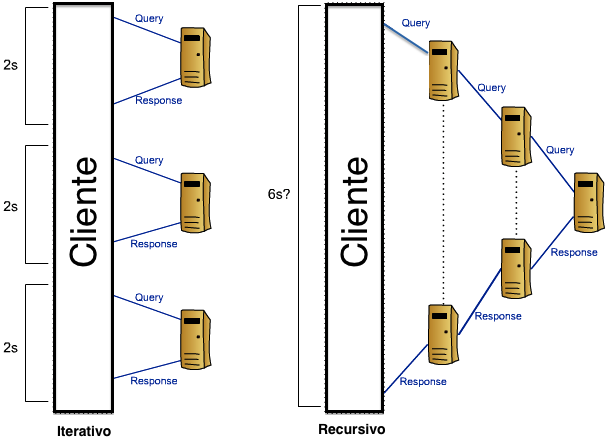
\includegraphics[width=0.7\textwidth]{figures/datagram-timing}
    \caption{Consulta iterativa e consulta recursiva}
    \label{consultas}
\end{figure}

Alguns conceitos introduzidos na especificação \cite{rfc1035} foram utilizados no
protocolo proposto, batizado de \textit{Fully Distributed Name Service - Service
Discovery} (FDNS-SD), como tradução reversa, tipos de registros (apesar de utilizar
diferentes tipos) e resolução recursiva de nomes -- isto é, o nó que pediu a
tradução recebe uma resposta ou uma mensagem de erro, em contrapartida à resolução
iterativa, em que o nó solicitante pode receber um novo endereço para enviar uma
nova solicitação de requisição (figura \ref{consultas}).

Outros conceitos definidos por \cite{rfc1035} foram descartados por se mostrarem
inapropriados ao tipo de rede na qual estão inseridos. Como a rede é dinâmica e
intrinsicamente volátil, não faz sentido usar um arquivo de configuração estático
como o \textit{Masterfile}. De fato, uma das características das redes MANET é a
auto-configuração, portanto o conceito mais natural para ser usado no protocolo
é o \textit{Zeroconf} \cite{zeroconf}. A hierarquia em árvore, por exigir servidores
confiáveis e com muitos recursos, também foi descartada para a construção do
FDNS-SD, e por consequência estruturas dependentes da árvore também foram eliminadas,
como TLDs e SLDs.

Existem conceitos ainda que foram modificados para se adaptarem ao novo ambiente
no qual o protocolo pretende atuar. A exemplo, o conceito de tipos de registros.
Na definição do DNS são descritos os tipos de registros, e em cada consulta é
possível especificar o tipo que é desejado na resposta, como tipo A para endereços,
MX para servidores de e-mail e PTR para ponteiros para outros servidores \cite{rfc1035}.
Esses tipos serão usados no FDNS-SD para possibilitar descoberta de serviço; de
fato, a própria tradução de nomes é tratada como mais um serviço disponível. O
FDNS-SD propõe uma nova visão sobre o serviço de nomes, pretendendo deixá-lo mais
adequado às restrições e exigências de uma MANET.

\subsection{Estrutura da proposta}

Este documento está organizado em quatro capítulos. O capítulo 2 analisa o estado
dos protocolos que existem hoje para resolução de nomes em MANETS, explicando o
funcionamento e apresentando os pontos fortes e fracos de cada protocolo.

O terceiro capítulo descreve a proposta de um novo protocolo completamente
distribuído para tradução de nomes e descoberta de serviços, incluindo os
algoritmos das tarefas executadas e as possibilidades de traduções. Posteriormente
algumas regras sobre conflitos de nomes e desconexão da rede são apresentadas.

O último capítulo apresenta a estratégia proposta para testes. Esse capítulo
explica o funcionamento da plataforma que será usada e por que foi escolhido um
emulador de rede ao invés de um simulador.